\documentclass{beamer}
\usepackage[frenchb]{babel}
\usepackage[utf8]{inputenc}
\usepackage[T1]{fontenc}
\usepackage{babel}
\usepackage{graphicx}
\usepackage{amsmath}
\usepackage{caption}
\usepackage{subcaption}
\usepackage{siunitx}
\usepackage{textcomp}
\usepackage{xcolor}
\usepackage[T1]{fontenc}
\usepackage[utf8]{inputenc}
\usepackage{tikz}
\usetikzlibrary{quotes,angles,calc,intersections,babel,through,backgrounds,angles,positioning}
\usepackage{rotating}

\usetheme{Warsaw}

\title[Goutte soufflée]{Goutte soufflée : croissance et dynamique d'une goutte cisaillée par un écoulement d'air\xspace}
\author{BESSENG A IREH Guy Raymond}
\institute[]{Université Paul Sabatier}
\date{21 Mars 2018}
\setbeamertemplate{caption}{\raggedright\insertcaption\par}
\addtobeamertemplate{navigation symbols}{}{%
    \usebeamerfont{footline}%
    \usebeamercolor[fg]{footline}%
    \hspace{1em}%
    \insertframenumber/\inserttotalframenumber
}
\begin{document}

\maketitle
%************************************************
\section{Introduction}\label{sec:introduction}
%************************************************
\begin{frame}
\frametitle{Introduction}
\begin{center}
\includegraphics[height=0.2\linewidth]{./image/test628.jpg} \\ 
\end{center}
\end{frame}


%************************************************
\section{Couche limite}\label{sec:couche}
%************************************************
\begin{frame}
\frametitle{Hypothèses}
\begin{itemize}
\item Écoulement bidimensionnel, stationnaire
\item $u \sim U$, $v \sim V$, $x \sim L$, $y \sim \delta$
\item $\frac{\delta}{L} << 1$
\item $F_{visqueux} \sim F_{inertiel}$
\end{itemize}
\begin{align}	
	\frac{\partial u}{\partial x} 
	+
	\frac{\partial v}{\partial y} 
	&= 0 \\
	u\frac{\partial u}{\partial x} + 
	v\frac{\partial u}{\partial y} 
	&= - \frac{1}{\rho}
	\frac{\partial p}{\partial  x} +
	\nu
	\frac{\partial^{2} u}{\partial  y^{2}} \\
	\frac{\partial p}{\partial y} 
	&= 0
\end{align}
\end{frame}

%************************************************
\subsection{Couche limite de Blasius}\label{sub:Blasius}
%************************************************

\begin{frame}
\frametitle{Couche limite de Blasius}
\begin{itemize}
\item Hypothèse couche limite
\item Vitesse à l'infini constante et suivant $x$
\end{itemize}
On pose :

\begin{align*}
	u(x,y) &= 
	\frac{\partial \varphi}{\partial y} \\
	v(x,y) &= - 
	\frac{\partial \varphi}{\partial x}
\end{align*}

Changement de variable :

\begin{align*}
	\eta &= y \sqrt{\frac{U}{\nu x }} \\
	\varphi &= \sqrt{2\nu U x} f(\eta)
\end{align*}
\end{frame}

\begin{frame}
\frametitle{Couche limite de Blasius}
Équation de  Couche limite de Blasius :
\begin{equation}	
	\frac{d^{3}f}{d\eta^{3}} + \frac{1}{2}f\frac{d^{2} f}{d\eta^{2}} = 0
\end{equation}
Avec les conditions aux limites :
\begin{align}
	u(x,0) &= 0 &\Rightarrow &&
	\left.
	\frac{d f}{d \eta}     \right|_{\eta = 0} &= 0
	\\
	v(x,0) &= 0 &\Rightarrow &&
	f(0) &= 0
	\\
	u(x,\infty) &= U &\Rightarrow &&
	\left.
	\frac{d f}{d \eta} \right|_{\eta = \infty} &= 1
\end{align}
\end{frame}
%************************************************
\subsection{Comparaisons Blasius et expérience}\label{sec:comparaison}
%************************************************
\begin{frame}
\frametitle{Couche limite de Blasius}
\begin{equation}
	\delta_{1}(x) = 
	\int_{0}^{^\infty}
	\left(
	1 - 
	\frac{u}{U}
	\right)
	dy
	\approx \frac{1.72x}{\sqrt{Re_{x}}}
\end{equation}

\begin{equation}
	\delta_{2}(x) = 
	\int_{0}^{^\infty}
	\frac{u}{U}
	\left(
	1 - 
	\frac{u}{U}
	\right)
	dy
	\approx \frac{0.664x}{\sqrt{Re_{x}}}
\end{equation}

\begin{equation}
	C_{f}(x) =
	\frac{2\tau_{y=0}}{\rho U^{2}} =
	\frac{2\nu}{U^{2}}
	\left.
	\frac{\partial u}{\partial y}
	\right|_{y = 0} \approx \frac{0.664}{\sqrt{Re_{x}}}
\end{equation}
\end{frame}

\begin{frame}
\frametitle{Couche limite de Blasius : Comparaisons Blasius et expérience}
\begin{equation*}
	x = 0.55m,~Re_{x} = \frac{Ux}{\nu},~
	\nu = 1.5e-5 m^{2}.s^{-1}~~\text{à}~~T = 25^{o}C
\end{equation*}

\begin{table}[ht]
	\centering
	\begin{tabular}{cc}
		\hline\\
		$U(m/s)$ & Reynolds\\
		\hline
   15 & 550000.00\\
   20 & 733333.33\\
   24 & 880000.00\\
   28 & 1026666.7
	\end{tabular}
	\caption{Nombre de Reynolds $Re_{x}$}
\end{table}
\end{frame}

\begin{frame}
\frametitle{Couche limite de Blasius : Comparaison $\delta_{1}$ Blasius et expérience}
\begin{table}[ht]
	\centering
	\begin{tabular}{cccc}
		\hline\\
		$U(m/s)$ & $\delta_{1Blasius}(mm)$ &
		$ \delta_{1Experience}(mm)$ & 
		 erreur relative\\
		\hline
		15   & 1.27   & 1.24   & 2.69\%\\
		20   & 1.11   & 1.10   & 0.61\%\\
		24   & 1.02   & 0.99   & 3.13\%\\
		28   & 0.96   & 0.95   & 1.55\%
	\end{tabular}
	\caption{Comparaison épaisseur de déplacement $\delta_{1}$}
\end{table}
\end{frame}

\begin{frame}
\frametitle{Couche limite de Blasius : Comparaison $\delta_{2}$ Blasius et expérience}
\begin{table}[ht]
	\centering
	\begin{tabular}{cccc}
		\hline\\
		$U(m/s)$ & $\delta_{2Blasius}(mm)$ &
		$ \delta_{2Experience}(mm)$ & 
		 erreur relative\\
		\hline
   15 & 0.49   & 0.47   & 3.64\%\\
   20 & 0.43   & 0.41   & 4.62\%\\
   24 & 0.40   & 0.37   & 6.08\%\\
   28 & 0.37   & 0.35   & 6.92\%
	\end{tabular}
	\caption{Comparaison épaisseur de quantité de mouvement $\delta_{2}$}
\end{table}
\end{frame}

\begin{frame}
\frametitle{Couche limite de Blasius : Comparaison $C_{f}$ Blasius et expérience}
\begin{table}[ht]
	\centering
	\begin{tabular}{cccc}
		\hline\\
		$U(m/s)$ & $C_{fBlasius}$ &
		$ C_{fExperience}$ & 
		 erreur relative\\
		\hline
   15 & 8.92e-04   & 9.19e-04   & 2.89\%\\
   20 & 7.77e-04   & 7.67e-04   & 1.31\%\\
   24 & 7.20e-04   & 7.33e-04   & 1.85\%\\
   28 & 6.75e-04   & 6.67e-04   & 1.26\%
	\end{tabular}
	\caption{Comparaison coefficient de frottement $C_{f}$}
\end{table}
\end{frame}

\begin{frame}
\frametitle{Couche limite de Blasius : Comparaison profil Blasius et expérience}
\begin{figure}[ht]
	\centering
	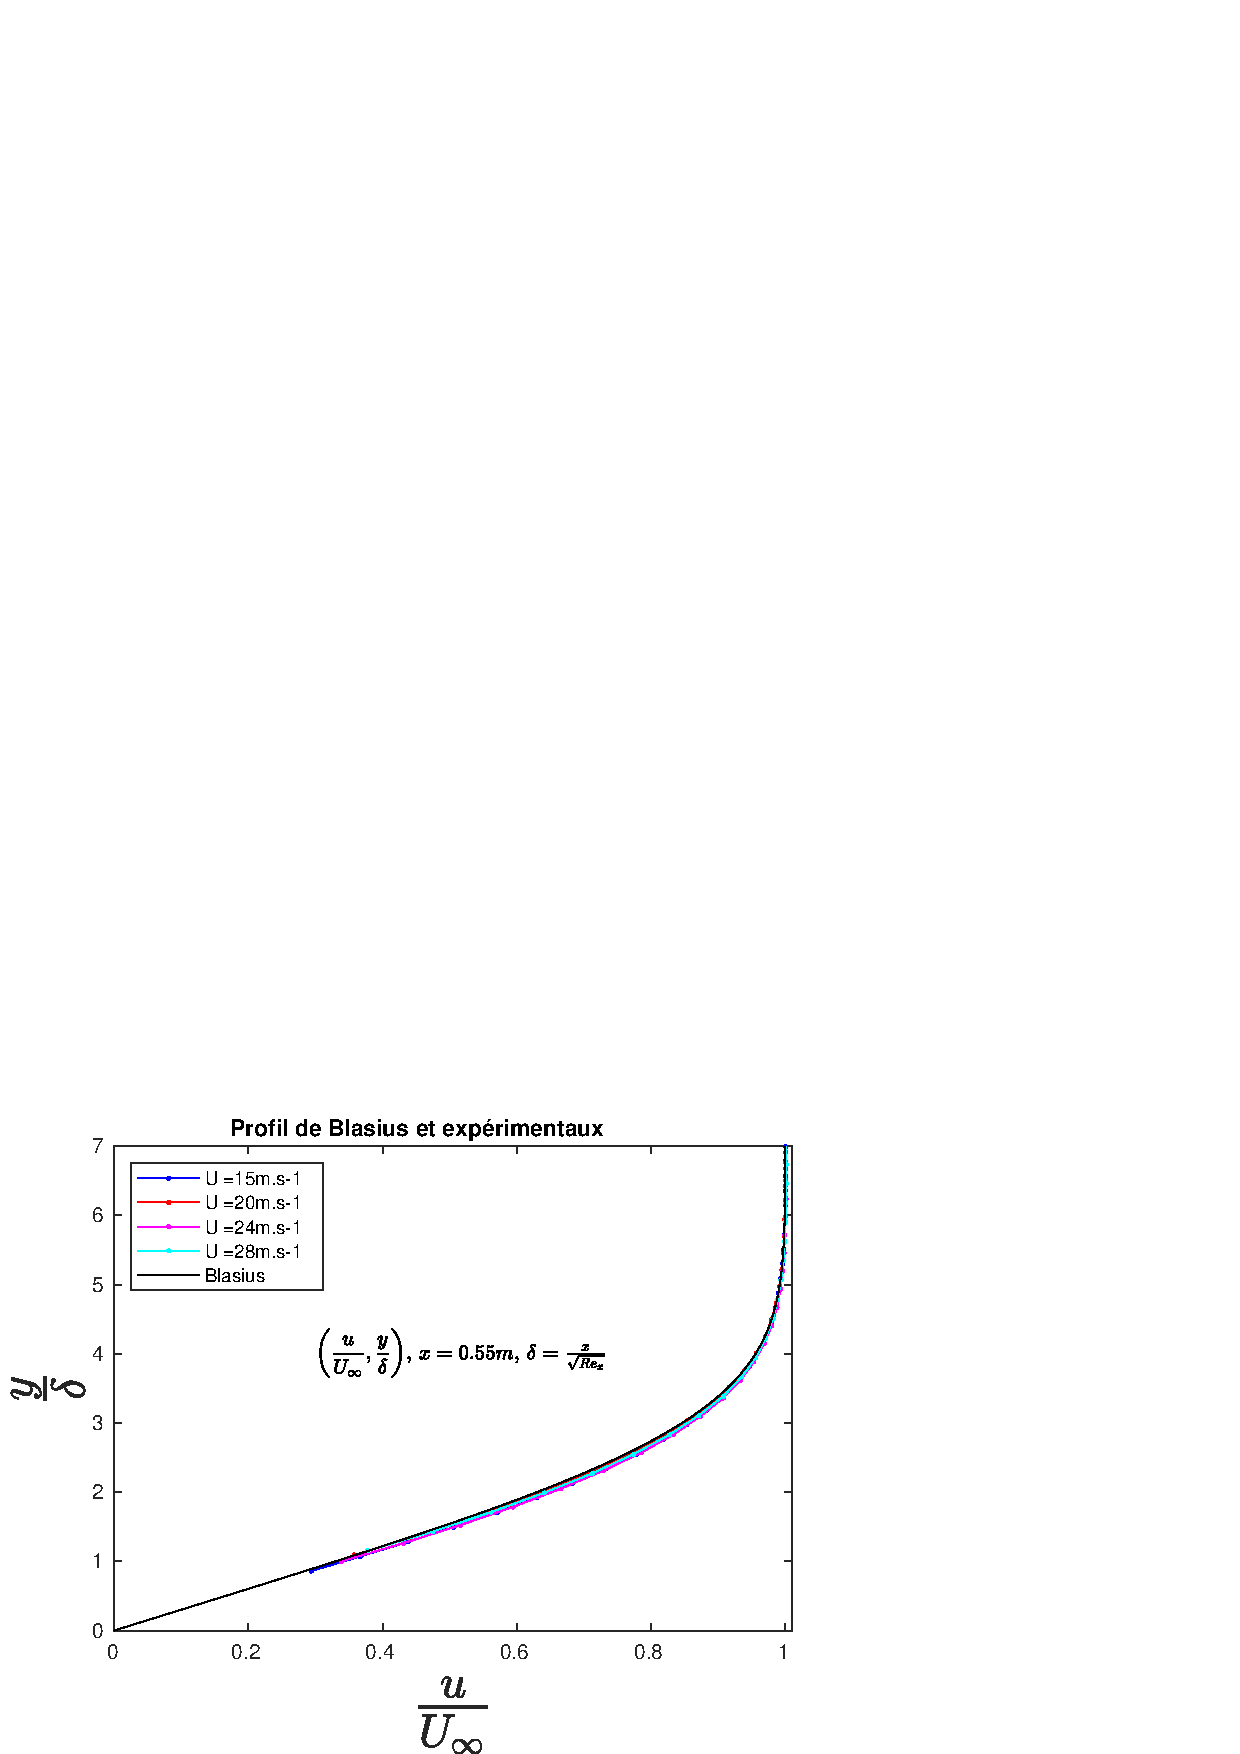
\includegraphics[scale = 0.5]{./image/Bla.png}
	\caption{Profil de Blasius et expérimentaux}
\end{figure}
\end{frame}

%************************************************
\section{Capillarité}\label{sec:capillarite}
%************************************************


%************************************************
\section{Expériences}\label{sec:experience}
%************************************************
\begin{frame}
\frametitle{Dispositif expérimental : Camera, surface et écran à laser}
\begin{figure}[!hb]
\centering
	\includegraphics[width = 0.4\linewidth]{./image/Surface.jpg}
	\caption{Camera, surface et écran à laser}
	\label{fig:Plan}
\end{figure}
\end{frame}


\begin{frame}
\frametitle{Dispositif expérimental : Ecran d'observation}
\begin{figure}[!hb]
\centering
	\includegraphics[width = 0.5\linewidth]{./image/Ecran.jpg}
	\caption{Ecran d'observation}
	\label{fig:Ecran d'observation}
\end{figure}
\end{frame}

\subsection{Paramètres mesurés}
\begin{frame}
\frametitle{Paramètres mesurés}
\begin{figure}[!ht]
	\centering
	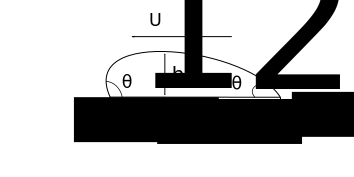
\includegraphics[scale = 0.8]{./image/rrgou2.png}
	\caption{Paramètres mesurés}
\end{figure}
\end{frame}

\begin{frame}
\frametitle{Example de mesure}
\begin{figure}[!ht]
	\centering
	\includegraphics[scale = 0.5]{./image/crop_tvitesse=28_volume=003.png}
	\caption{Goutte d'eau de volume $0.03$ml avec: \\$U = 0$, $\theta_{1} = \ang{45}$, $\theta_{2} = \ang{50.17}$, $x_{1} = 14.66mm$, $x_{2} = 6.77mm$,\\ $d = 7.89mm$, $h = 4.86mm$ et $x_{h} = 11.08mm$}
\end{figure}
\end{frame}

\subsection{Résultats}

\begin{frame}
\frametitle{Résutats}
\begin{figure}[!ht]
	\centering
		\includegraphics[width=\linewidth]{./image/v=24_vol=004_xaxrd.jpg}
		\caption{$\textcolor{blue}{x_{a}}$,
		$\textcolor{red}{x_{r}}$, $\textcolor{yellow}{d}$, 
		$U_{\infty}=24m.s^{-1}$, \\
                volume =$0.04ml$}
		\label{fig:entre_xaxrd}
		 \end{figure}
\end{frame}
\begin{frame}
\frametitle{Analyse des résutats : $\textcolor{blue}{\theta_{a}}$,
		$\textcolor{red}{\theta_{r}}$ pour $U_{\infty}=24m.s^{-1}$ et volume =$0.04ml$}
\begin{figure}[!ht]
		\includegraphics[width=\linewidth]{./image/v=24_vol=004_oaor.jpg}
		\caption{$\textcolor{blue}{\theta_{a}}$,
		$\textcolor{red}{\theta_{r}}$, $U_{\infty}=24m.s^{-1}$, volume =$0.04ml$}
		\label{fig:entre_oaor}
 \end{figure}
\end{frame}
\begin{frame}
\frametitle{Analyse des résutats : oscillations}
\begin{figure}[!ht]
		\includegraphics[width = 0.35\linewidth]{./image/test.jpg}\\
		\includegraphics[width = 0.35\linewidth]{./image/test400.jpg}\\
		\includegraphics[width = 0.35\linewidth]{./image/test626.jpg}\\
		\includegraphics[width = 0.35\linewidth]{./image/test627.jpg}\\
		\includegraphics[width = 0.35\linewidth]{./image/test628.jpg}\\
		\includegraphics[width = 0.35\linewidth]{./image/test629.jpg}
	\caption{$U_{\infty}=20m.s^{-1}$, de haut en bas nous avons :\\
	$t = ~0s,~8s,~12.52s,~12.54s,~12.58s$}
		\label{fig:test}
\end{figure}
\end{frame}

\begin{frame}
\frametitle{Analyse des résutats : $d$ pour $U_{\infty}=20m.s^{-1}$}
\begin{figure}[!ht]
        \centering
		\includegraphics[width = \linewidth]{./image/v=20d.jpg}
	\caption{$d$, $U_{\infty}=20m.s^{-1}$}
		\label{fig:v=20d}
\end{figure}
\end{frame}

\begin{frame}
\frametitle{Analyse des résutats : $\theta_{a}$ pour $U_{\infty}=20m.s^{-1}$}
\begin{figure}[!ht]

	\includegraphics[width = \linewidth]{./image/v=20oa_2.jpg}
	\caption{$\theta_{a}$, $U_{\infty}=20m.s^{-1}$}
		\label{fig:v=20oa_2}
\end{figure}
\end{frame}

\begin{frame}
\frametitle{Analyse des résutats : $\theta_{r}$ pour $U_{\infty}=20m.s^{-1}$}
\begin{figure}[!ht]
        \centering
	\includegraphics[width = \linewidth]{./image/v=20or_2.jpg}
	\caption{$\theta_{r}$, $U_{\infty}=20m.s^{-1}$}
		\label{fig:v=20or_2}
\end{figure}
\end{frame}

\begin{frame}
\frametitle{Analyse des résutats : $x_{max}$ pour $U_{\infty}=20m.s^{-1}$}
\begin{figure}[!ht]
        \centering
	\includegraphics[width = \linewidth]{./image/v=20xm.jpg}
	\caption{$x_{max}$, $U_{\infty}=20m.s^{-1}$}
		\label{fig:v=20xm}
\end{figure}
\end{frame}

\begin{frame}
\frametitle{Analyse des résutats : $y_{max}$ pour $U_{\infty}=28m.s^{-1}$}
\begin{figure}[!ht]
        \centering
	\includegraphics[width = 0.9\linewidth]{./image/v=20ym.jpg}
	\caption{$y_{max}$, $U_{\infty}=28m.s^{-1}$}
		\label{fig:v=20ym}
\end{figure}
\end{frame}


\begin{frame}
\frametitle{Analyse des résutats : longueur $d$ avec et sans debit}
\begin{figure}[!ht]
        \centering
	\includegraphics[width = \linewidth]{./image/p=365_vol=006d.jpg}
	\caption{$d$ , volume $= 0.06ml$, vitesse $\approx 24.7m.s^{-1}$}
\label{fig:p=365_vol=006d}
\end{figure}
\end{frame}

\begin{frame}
\frametitle{Conclusion et perspectives}
\end{frame}

\begin{frame}
\frametitle{Questions}
  \center{Avez-vous des questions ?}
\end{frame}



\end{document}
